%!TEX root = ../report.tex

\chapter{Experimental Evaluation}
In the section \ref{analysis}, a primary analysis was conducted to evaluate the effects of various parameters used in a DMP, on the trajectory approximation. This analysis gave insights of capabilities, limitations and precautions that are needed to be taken while using a DMP. But to evaluate the entire \textit{Learning from Demonstration} framework, experiments are needed to be carried out on real robots. Numerous such experiments were conducted on KUKA YouBot and Toyota HSR, for evaluating the performance of DMP framework and proposed methodology. The experiments conducted on KUKA YouBot were mainly aimed at:
\begin{itemize}
	\item evaluating generalization ability of DMPs,
	\item evaluating performance of whole body motion control with DMPs,  
\end{itemize}
Two experiments were also conducted on Toyota HSR for:
\begin{itemize}
	\item demonstrating the easiness of porting above solution from one robot to another,
	\item evaluating performance of whole body motion control with DMP,
	\item sequencing two DMPs to grasp an object.
\end{itemize} 

\subsection{Experimental Setup}

\begin{tabular}{c c c}
	\textbf{Robot 1} & : & KUKA YouBot \\       
	\textbf{Robot 2} & : & Toyota HSR \\
	\textbf{Camera} & : & Asus Xtion Pro Live\\
	\textbf{Softwares and Libraries} & : & OpenCV 3.1.0 \\
	 & : & Robot Operating System (ROS) Kinetic \\
	 & : & OROCOS Kinematics and Dynamics library \\
	 Environment 1 & : & RoboCup@Work lab, C025 \\
	 Environment 2 & : & RoboCup@Home lab, C069
	 
	                                      
\end{tabular}
 

\subsection{Acquisition and Repetition of Dynamic Motion Primitives}

Aim of this experiment was to evaluate the ability of above proposed software architecture, of acquiring human demonstrations, learning the motion primitives, and repeat the motion primitives multiple times for different goals, in order to evaluate generalization ability of motion primitives for different end-effector goal positions (hereafter, goal always refer to end-effector goal position) and the ability of accurately executing the motion primitives. 

In this experiment, four different trajectories were demonstrated to the robot in task-space, motion primitives were learned and stored in the library. Then each motion primitive was used to generate trajectories with five different goals in task-space. Ten trials were conducted for each of the goals to check the repeatability. In each trial, the trajectory started from the same initial position. Lets discuss the experiments for each motion primitive, in detail. 

\begin{figure}[H]
	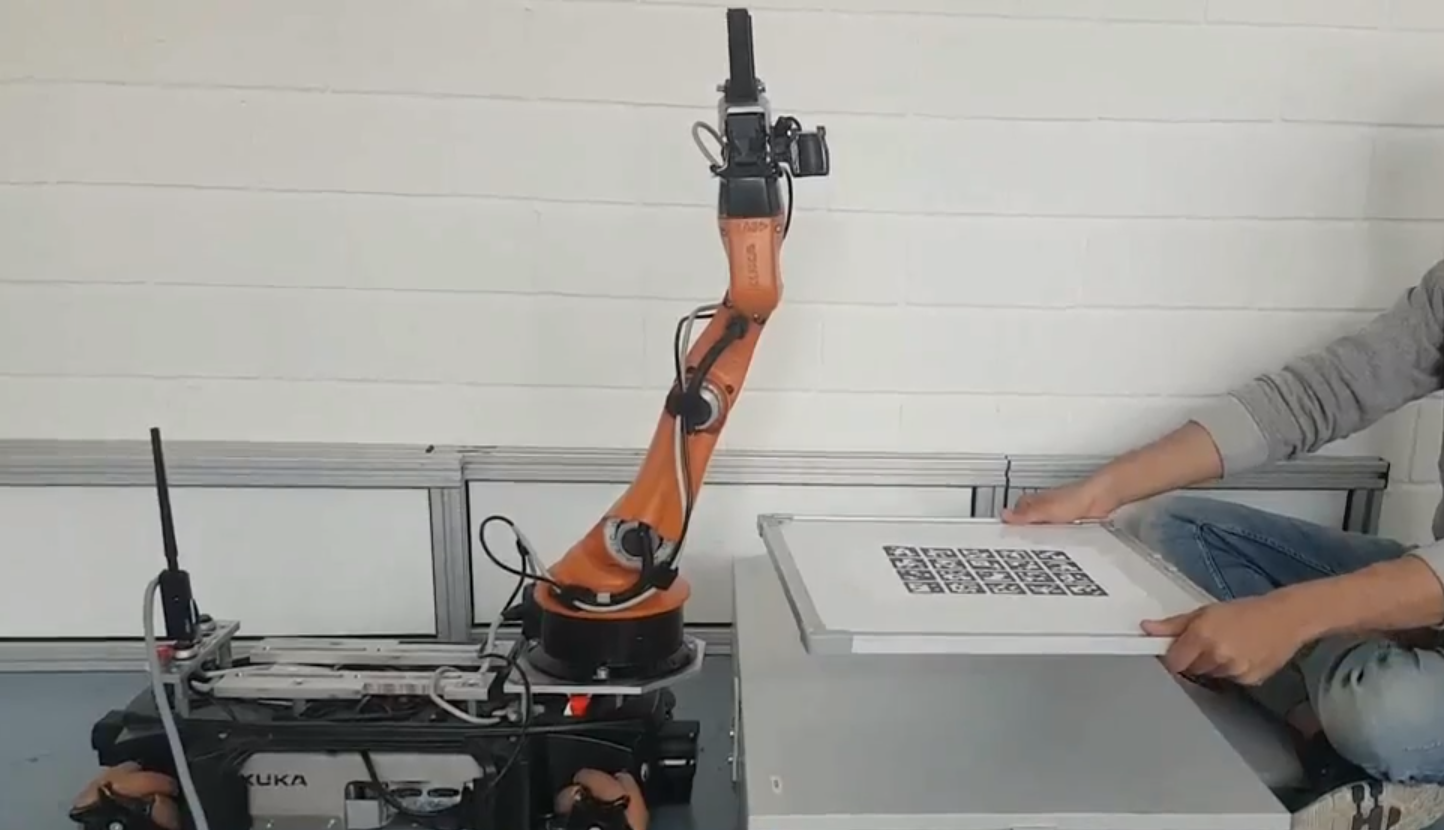
\includegraphics[width=\textwidth]{images/demo.png}
	\caption{Demonstration of the trajectory using arUco marker board}
	\label{fig:demo}
\end{figure}

\subsubsection{Inverted Parabolic Trajectory 1}
Fig. \ref{fig:inv_par_1} shows the inverted parabola like trajectories for five different goals. Figure contains both, the planned trajectories generated by the DMP and the trajectories executed by the robot. All the trajectories are generated from one motion primitive. 

\textbf{Experimental parameters:} \\
$n\_bfs$ = 50 \hspace{3cm}
$\tau$ = 10 \hspace{3cm}
$dt = 0.01$ \\
Initial position = [0.522, -0.058, 0.042]$m$ \\
Goal 1 = [0.537, 0.161, 0.044]$m$ \hspace{2cm}
Goal 2 = [0.508, 0.161, 0.044]$m$ \\
Goal 3 = [0.538, 0.131, 0.044]$m$ \hspace{2cm}
Goal 4 = [0.508, 0.181, 0.044]$m$ \\
Goal 5 = [0.568, 0.141, 0.044]$m$
\begin{figure}[H]
	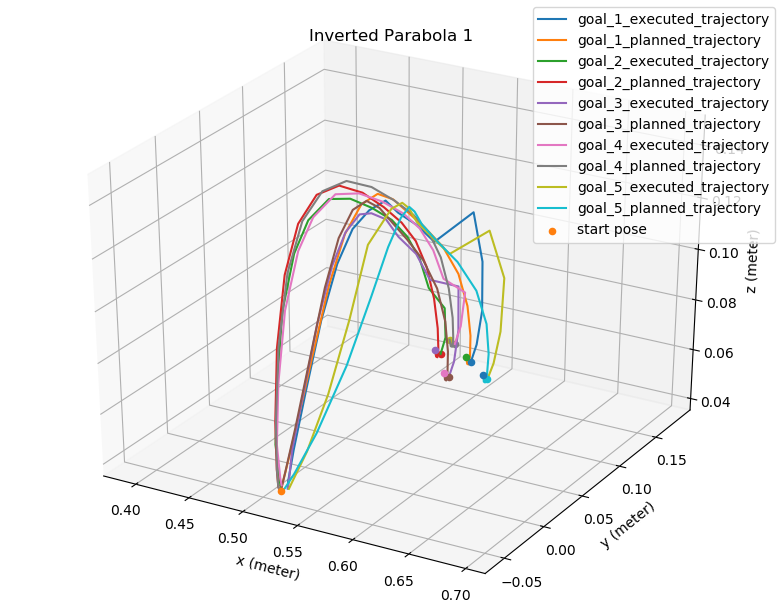
\includegraphics[width=\textwidth]{images/1/inv_par_1.png}
	\caption{Inverted parabolic trajectory 1}
	\label{fig:inv_par_1}
\end{figure}

In the figure, it can be observed that the executed trajectories differ from the planned ones, which suggest that the error is introduced by the trajectory controller as well as the joint velocity controllers in the robot. Despite of this, error was calculated as the normalized point-to-point error for the entire trajectory. In case of executed trajectories for goal 1 and goal 5, a sudden overshoot can be observed at end of the trajectory. This overshoot occurred because of this part of trajectory was out of the workspace of the manipulator. A degraded inverse kinematic solution is generated in such cases by the method described in the section \ref{IK}. Despite of this, end-effector was able to reach the goal position because of the position feedback used in trajectory executor. This situation particularly triggered the idea of using base motion and hence the whole body motion to execute the trajectories.  

\begin{figure}[H]
	\centering
	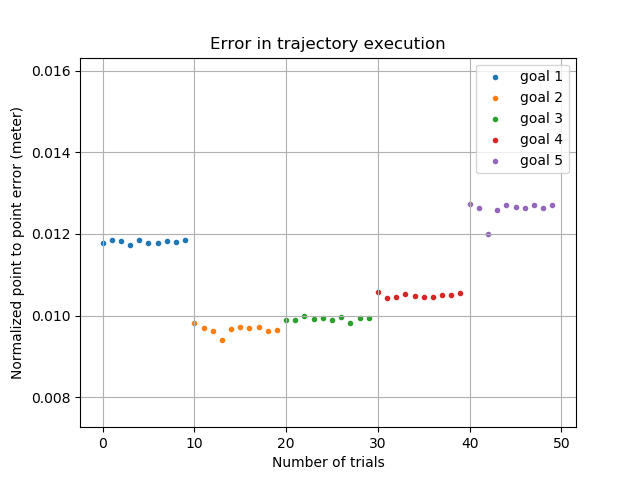
\includegraphics[scale=0.65]{images/1/inv_par_1_e.png}
	\caption{Error in the execution of trajectories}
	\label{fig:inv_par_1_e}
\end{figure}

Fig. \ref{fig:inv_par_1_e} shows the normalized point to point error in each executed trajectory calculated by eq. \ref{t_error}. 

\subsubsection{Inverted Parabolic Trajectory 2}

Figures \ref{fig:inv_par_2} and \ref{fig:inv_par_2_e} respectively show another inverted parabola like trajectory generalized for 5 different goals and the error in the execution of same over ten trials per goal. 

\textbf{Experimental parameters:} \\
$n\_bfs$ = 50 \hspace{3cm}
$\tau$ = 10 \hspace{3cm}
$dt = 0.01$\\
Initial position = [0.456, -0.234, 0.121]$m$ \\
Goal 1 = [0.496, 0.100, 0.089]$m$ \hspace{2cm}
Goal 2 = [0.476, 0.119, 0.058]$m$ \\
Goal 3 = [0.451, 0.149, 0.043]$m$ \hspace{2cm}
Goal 4 = [0.493, 0.179, 0.074]$m$ \\
Goal 5 = [0.493, 0.228, 0.089]$m$


\begin{figure}[H]
	\centering
	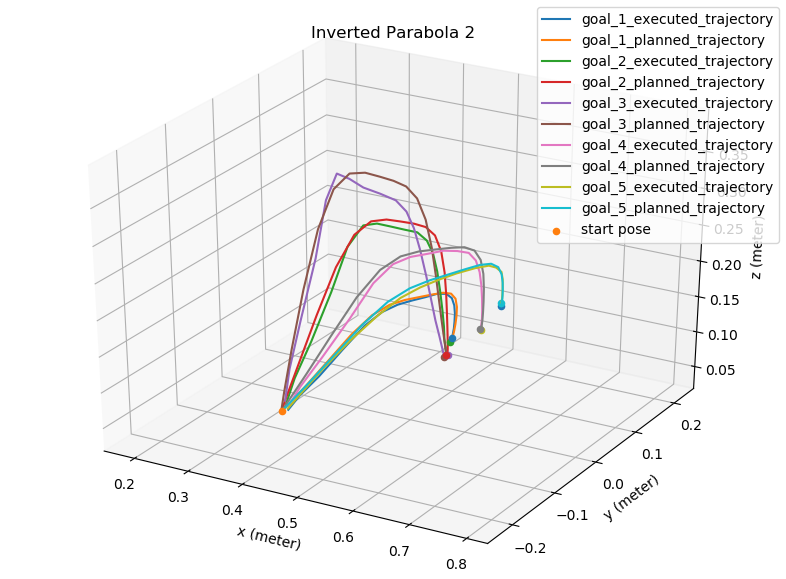
\includegraphics[scale=0.60]{images/1/inv_par_2.png}
	\caption{Inverted parabolic trajectory 2}
	\label{fig:inv_par_2}
\end{figure}


\begin{figure}[H]
	\centering
	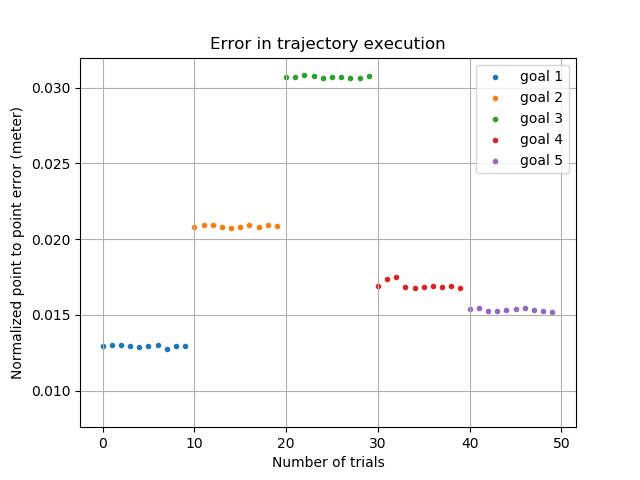
\includegraphics[scale=0.65]{images/1/inv_par_2_e.png}
	\caption{Error in the execution of trajectories}
	\label{fig:inv_par_2_e}
\end{figure}

\subsubsection{Inverted Parabolic Trajectory 3}


Trajectories in fig. \ref{fig:inv_par_3} show slightly different behavior. While executing these trajectories, a observation was made : if the sign of the difference between goal and the initial position (sign of ($g - y0$)) used in a DMP is opposite that of the trajectory from which the DMP was learned (sign of ($g_{demo} - y0_{demo}$)), the shape of the newly generated trajectory is mirrored. This can be observed from planned and executed trajectory for goal 2. 


\begin{figure}[H]
	\centering
	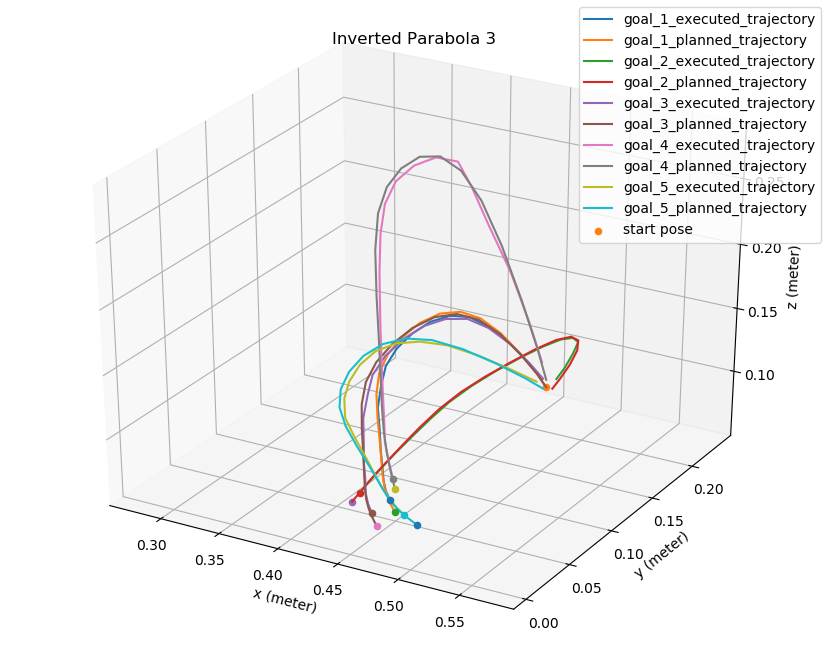
\includegraphics[scale=0.6]{images/1/inv_par_3.png}
	\caption{Inverted parabolic trajectory 3}
	\label{fig:inv_par_3}
\end{figure}

The reason behind this behavior can be found in eq. \ref{forcing_term}, where term ($g - y$) is multiplied to weighted sum of Gaussian functions to generate the forcing term $f$. Hence if the sign of ($g - y$) is opposite, then the forcing term also carries the opposite sign and generates the accelerations in opposite directions so that shape of the generated trajectory is mirrored. 

\textbf{Experimental parameters:} \\
$n\_bfs$ = 50 \hspace{3cm}
$\tau$ = 10 \hspace{3cm}
$dt = 0.01$\\
Initial position = [0.446, 0.230, 0.063]$m$ \\
Goal 1 = [0.470, 0.023, 0.074]$m$ \hspace{2cm}
Goal 2 = [0.434, 0.023, 0.074]$m$ \\
Goal 3 = [0.470, 0.003, 0.074]$m$ \hspace{2cm}
Goal 4 = [0.470, 0.023, 0.092]$m$ \\
Goal 5 = [0.488, 0.023, 0.068]$m$


Figure \ref{fig:inv_par_3_e} shows the error in the execution of above trajectories. 

\begin{figure}[H]
	\centering
	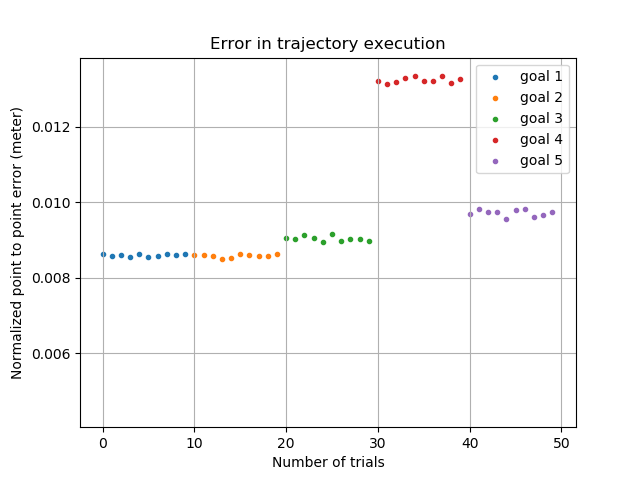
\includegraphics[scale=0.65]{images/1/inv_par_3_e.png}
	\caption{Error in the execution of trajectories}
	\label{fig:inv_par_3_e}
\end{figure}

\subsubsection{Step Function Trajectory}

Fig. \ref{fig:step_fun} shows the step function trajectories. This time, the step function like trajectory was demonstrated to the robot. Planned and executed trajectory for goal 2 is of special interest in this experiment. This trajectory was obtained by swapping the weights learned for DMPs in X and Y axis. It can be concluded from this experiment that, by combining DMPs learned in individual degrees of freedom, a new motion primitive can be synthesized. Another important observation in this experiment was on the use of time scaling factor $\tau$. For higher values of $\tau$, a overshoot was observed in the trajectory. 

\textbf{Experimental parameters:} \\
$n\_bfs$ = 50 \hspace{3cm}
$\tau$ = 10 \hspace{3cm}
$dt = 0.01$\\
Initial position = [0.5, -0.137, 0.05]$m$\\
Goal 1 = [0.500, 0.172, 0.129]$m$ \hspace{2cm}
Goal 2 = [0.561, 0.000, 0.129]\\
Goal 3 = [0.500, 0.172, 0.153]$m$ \hspace{2cm}
Goal 4 = [0.500, 0.204, 0.145]\\
Goal 5 = [0.500, 0.118, 0.089]

\begin{figure}[H]
	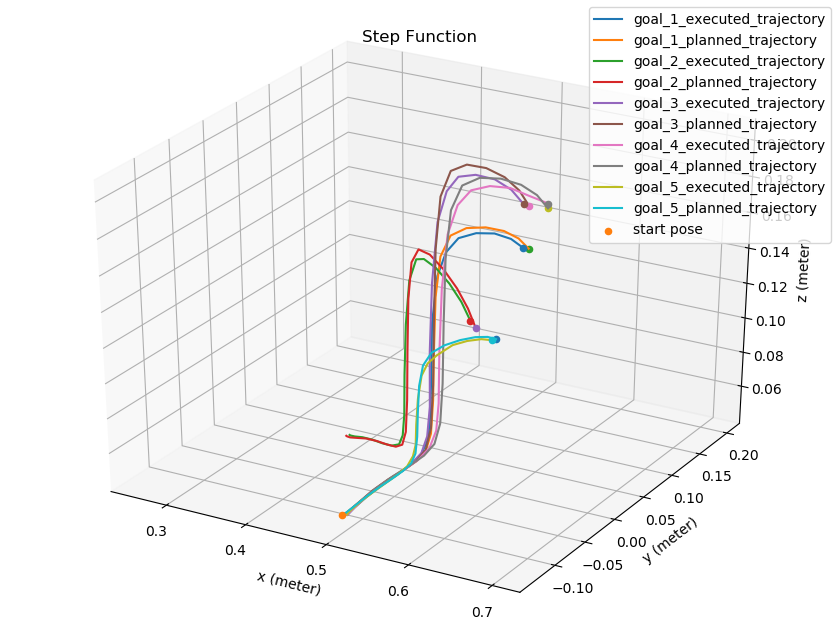
\includegraphics[width=\textwidth]{images/1/step.png}
	\caption{Step function trajectory}
	\label{fig:step_fun}
\end{figure}

Fig. \ref{fig:step_fun_e} shows the error in the execution of step function trajectories for different goals. 

\begin{figure}[H]
	\centering
	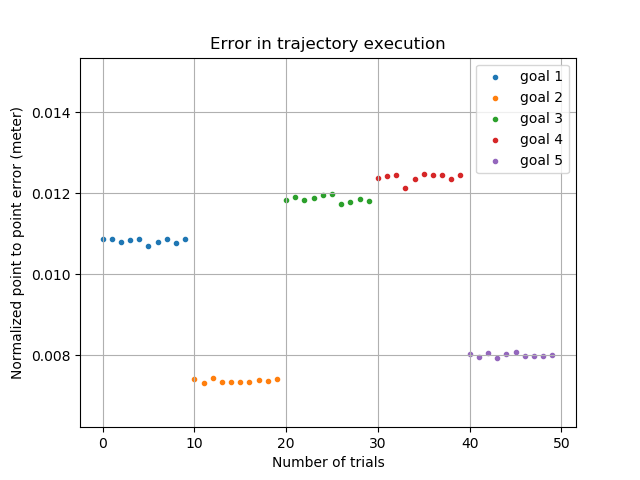
\includegraphics[scale=0.60]{images/1/step_e.png}
	\caption{Error in the execution of step function trajectories}
	\label{fig:step_fun_e}
\end{figure}

\subsubsection{Square Wave Trajectory}

An artificially generated square wave trajectory in X-Y plane (Z is constant) was learned using DMPs. Reason behind learning this particular trajectory was evaluate the ability to learn and execute motion with sharp turns. From earlier experience, the number of basis function was decided to be 500 because of the sharp turns which contribute to high frequency components. The controller, as expected, executed trajectory with oscillations at the corners of the path. These oscillations can be seen in fig. \ref{fig:square}. Because of high number of basis functions and low $\tau$, DMP generated a stable trajectory, but linear trajectory controller could not execute it perfectly; this marks the need of non-linear controller (torque controller) for more precise trajectory execution. However, the error in execution in trajectories is considerably low as seen in fig. \ref{fig:square_e}, hence for practical purposes, the controller's performance is satisfactory. 

A small peak along Z-axis can be observed on one of the corners of executed trajectory of goal 4; it occurred because the part of trajectory was near the boundary of dexterous workspace of the manipulator. As explained earlier, a degraded inverse kinematic solution was generated which led manipulator end-effector to deviate from the trajectory.


\begin{figure}[H]
	\centering
	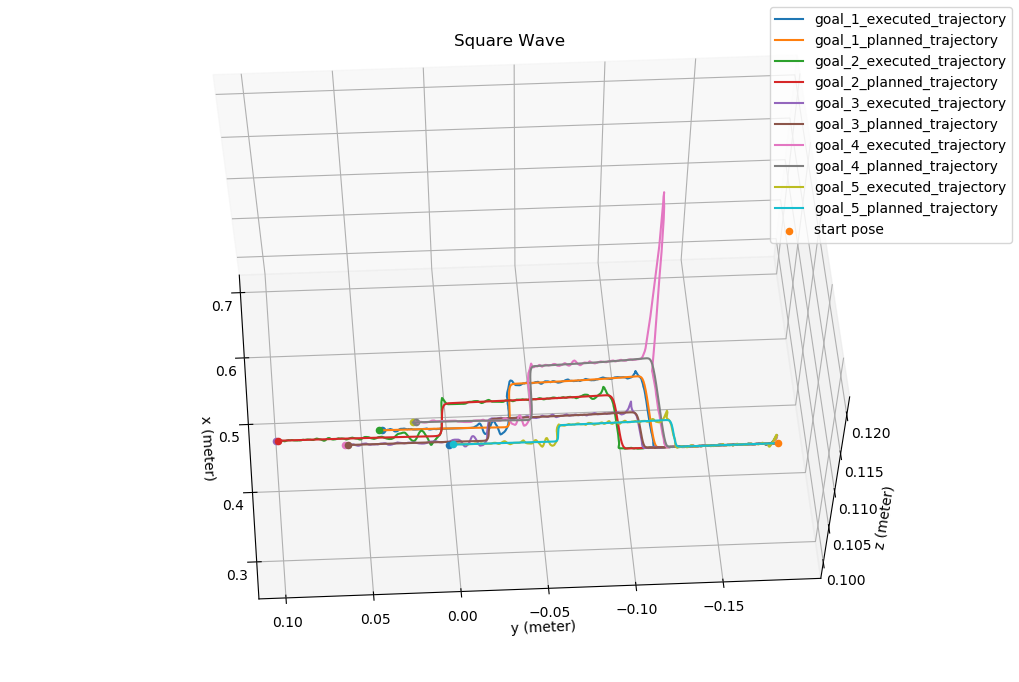
\includegraphics[scale=0.6]{images/1/square.png}
	\caption{Square wave trajectory}
	\label{fig:square}
\end{figure}


\begin{figure}[H]
	\centering
	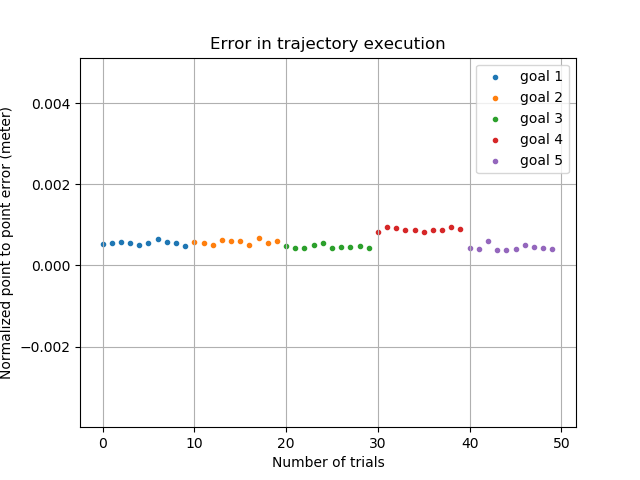
\includegraphics[scale=0.6]{images/1/square_e.png}
	\caption{Error in the execution of square wave trajectories}
	\label{fig:square_e}
\end{figure}

\subsection{Whole Body Motion Control on KUKA YouBot}

This experiment was conducted to demonstrate the ability of the proposed \textit{whole body motion control} architecture. 3 different trajectories were learned using DMP and used to generate the trajectories for five different task-space goals which are not in dexterous workspace of manipulator. Ten trials were conducted for each goal. 

Aim of this experiment was to evaluate the trajectory tracking ability with whole body motion control algorithm in the presence of uncertainties like slip in the wheels of mobile base, friction provided by the floor, etc. Apart form the parameters used in the DMP, motion is now affected by the parameters used in the whole body motion control. 

\begin{figure}[H]
	\centering
	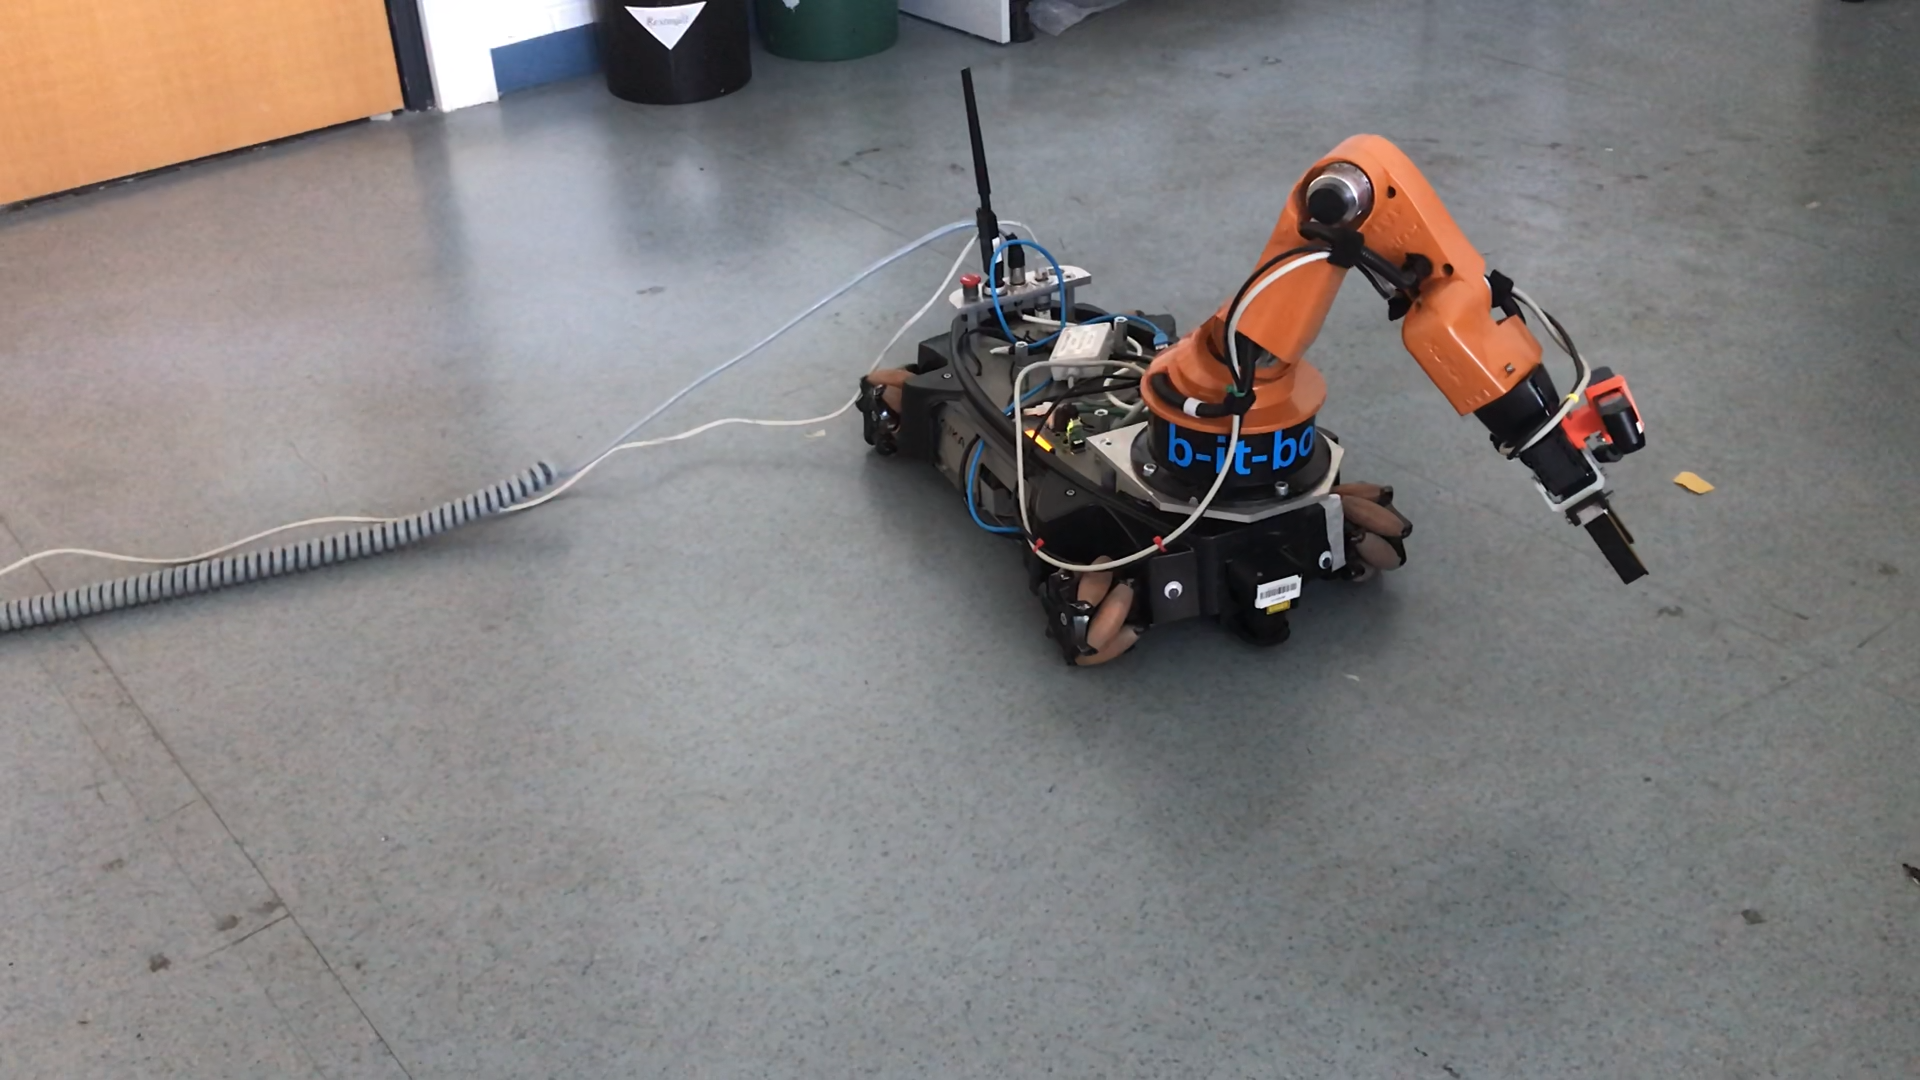
\includegraphics[scale=0.2]{images/wbc_kuka.png}
	\caption{KUKA YotBot performing whole body motion}
	\label{fig:wbc_kuka}
\end{figure}


\subsubsection{Inverted Parabolic Trajectory}

Same as the first experiment, inverted parabolic trajectory was demonstrated to the robot, learned and generalized for five different goals which are out of the dexterous workspace of the robot manipulator. It should be noted that the only internal wheel encoder feedback was used while motion execution hence it is not possible to compensate the error introduced by imprecise motion of the base. Hence, even if the error in execution as per the fig. \ref{fig:inv_par_wbc_e} is small, actual motion was not precise in global frame of reference. It was evident from the visual observation that the end-effector positions, after finishing motion for same goal in two different trials, were not same.  

\textbf{Experimental parameters:} \\
$n\_bfs$ = 500 \hspace{3cm}
$\tau$ = 10 \hspace{3cm}
$dt = 0.01$\\
Initial position = [0.423, -0.173, 0.110]$m$ \\
Goal 1 = [0.229, 0.206, 0.062]$m$ \hspace{2cm}
Goal 2 = [0.439, 0.358, 0.062]$m$\\
Goal 3 = [0.492, 0.446, 0.062]$m$\hspace{2cm}
Goal 4 = [0.535, 0.412, 0.062]$m$\\
Goal 5 = [0.639, 0.510  0.062]$m$

\begin{figure}[H]
	\centering
	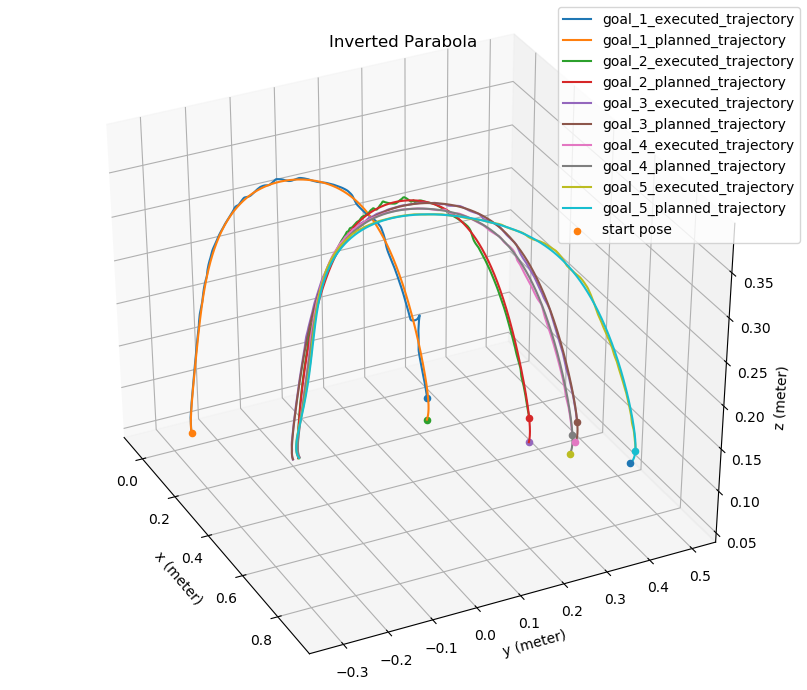
\includegraphics[scale=0.6]{images/2/inv_par.png}
	\caption{Inverted parabolic trajectory}
	\label{fig:inv_par_wbc}
\end{figure}

\begin{figure}[H]
	\centering
	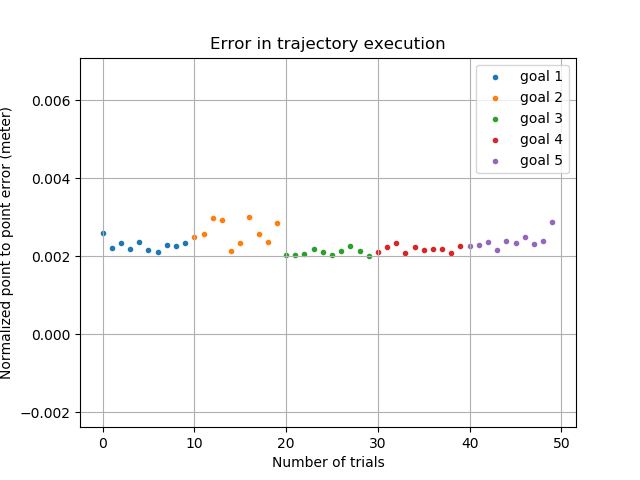
\includegraphics[scale=0.6]{images/2/inv_par_e.png}
	\caption{Error in the execution trajectories}
	\label{fig:inv_par_wbc_e}
\end{figure}


\subsubsection{Square Wave Trajectory 1}

A square wave like trajectory was demonstrated and learn. It was also generalized for five different goals. Interesting fact in this experiment was the imprecise execution of trajectories near the joint limits as observed in executed trajectories for goal 1 and 5 in fig. \ref{fig:square_wbc}. Another important observation is, when the goal separation, ($g - y0$), where $y0$ is the initial position, in certain degree of freedom is 0, then DMP does not take off i.e. does not leave the initial position. In planned and executed trajectories for goal 4, it can be observed that the goal separation in X-axis is 0, hence the shape of the trajectory is not as expected. The reason behind such behavior is the that the forcing term $f$ which responsible for the shape of the trajectory is scaled by goal separation (refer eq. \ref{forcing_term}) and hence the 0 goal separation makes $f$ equal to 0, at all the time.  

\textbf{Experimental parameters:} \\
$n\_bfs$ = 500 \hspace{3cm}
$\tau$ = 10 \hspace{3cm}
$dt = 0.01$\\
Initial position = [0.45, -0.116, 0.11]$m$ \\
Goal 1 = [0.394, 0.374, 0.11]$m$ \hspace{2cm}
Goal 2 = [0.416, 0.392, 0.11]$m$\\
Goal 3 = [0.387, 0.493, 0.11]$m$\hspace{2cm}
Goal 4 = [0.445, 0.341, 0.11]$m$\\
Goal 5 = [0.342, 0.540, 0.11]$m$

\begin{figure}[H]
	\centering
	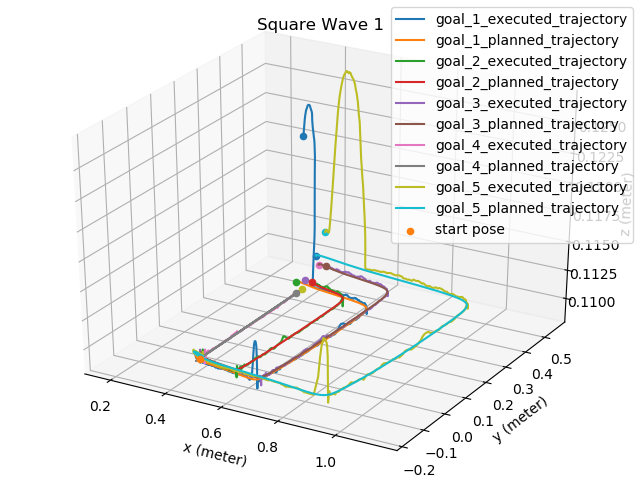
\includegraphics[scale=0.75]{images/2/square.png}
	\caption{Square wave trajectory 1 (WBC)}
	\label{fig:square_wbc}
\end{figure}


\begin{figure}[H]
	\centering
	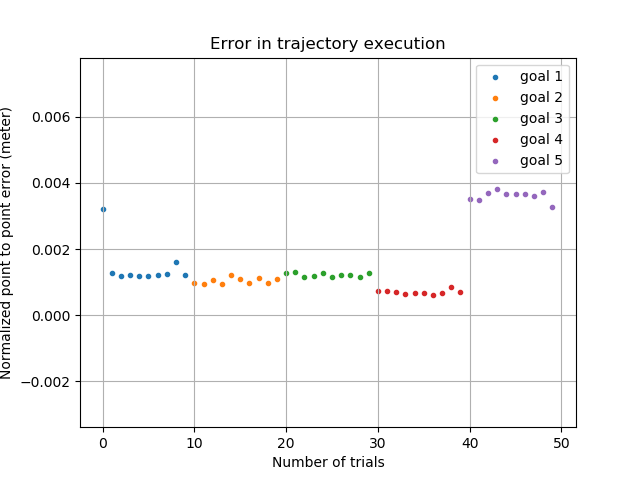
\includegraphics[scale=0.65]{images/2/square_e.png}
	\caption{Error in execution of trajectories}
	\label{fig:square_wbc_e}
\end{figure}

\begin{figure}[H]
	\centering
	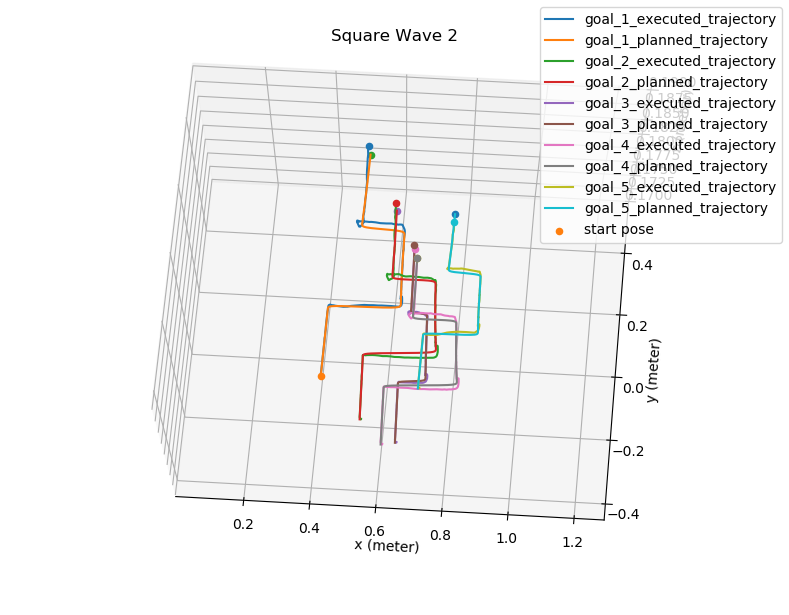
\includegraphics[scale=0.58]{images/2/wbc.png}
	\caption{Square wave trajectory 2 (WBC)}
	\label{fig:square_wbc_2}
\end{figure}


\begin{figure}[H]
	\centering
	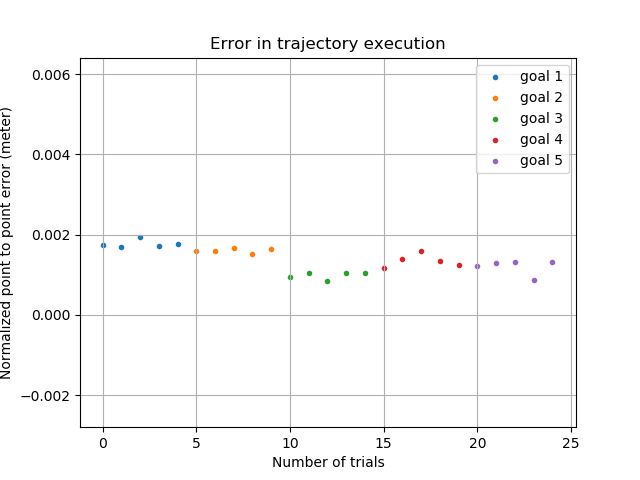
\includegraphics[scale=0.6]{images/2/wbc_e.png}
	\caption{Error in execution of trajectories}
	\label{fig:square_wbc_2_e}
\end{figure}
Fig. \ref{fig:square_wbc_2} and \ref{fig:square_wbc_2_e} respectively show another square wave like trajectory execution and error in the execution.


\subsubsection{Discussion}

This was first experiment conducted on the robot which helped us get insights of the problems in using DMPs on real robot. Some important observation were made:
\begin{itemize}
	\item If some part of a trajectory is out of the dexterous workspace or near its limits (e.g. the goal position is at the limits of the workspace), the motion is unpredictable due to degraded inverse kinematics solutions; this limits the ability to generalize a learned primitive.
	\item A similar observation holds near the joint limits.
	\item If the demonstrated trajectory has initial and final values of position on particular axis that are practically equal to each other, varying goal on that axis creates infeasible resulting trajectories; this primitive is thus limited to scenarios in which the initial and final position are the same on that axis. For example, if a motion primitive is learned for picking an object and placing it elsewhere at same height ($z_{initial}$ = $z_{goal}$), and used for placing object at higher heights, it can create potentially dangerous trajectories. Reason behind this behavior is the scaling term ($g - y_0$) in eq. \ref{forcing_term}; while learning if this scaling term is practically zero, and while generating new trajectory, it is relatively big (sign of this term does not matter), shape of the DMP in that particular direction is scaled.    
	\item Increasing $\tau$ too much (e.g. 100) causes overshoots at sharp turns.
	\item At sharp turns, oscillations around the trajectory occur because of linear trajectory controller. 
	\item For learning motion with sharp turns, use of high number of basis functions is desired. 
	\end{itemize}

\section{Dynamic Motion Primitives on Toyota HSR}

For demonstrating the usefulness of DMPs in RoboCup@Home scenario, the \textit{Learning from Demonstration} framework was adopted for Toyota HSR and two experiments were conducted:

\begin{enumerate}
	\item Sequencing two DMPs for pick and place task
	\item Grasping an object 
\end{enumerate} 

In these experiments, obstacles were present in the environment and thus the motion of the base was restricted. Hence feedback form the laser scanners was used in the whole body motion control.   

\subsection{Sequencing two DMPs for pick and place task}
\begin{figure}[H]
	\centering
	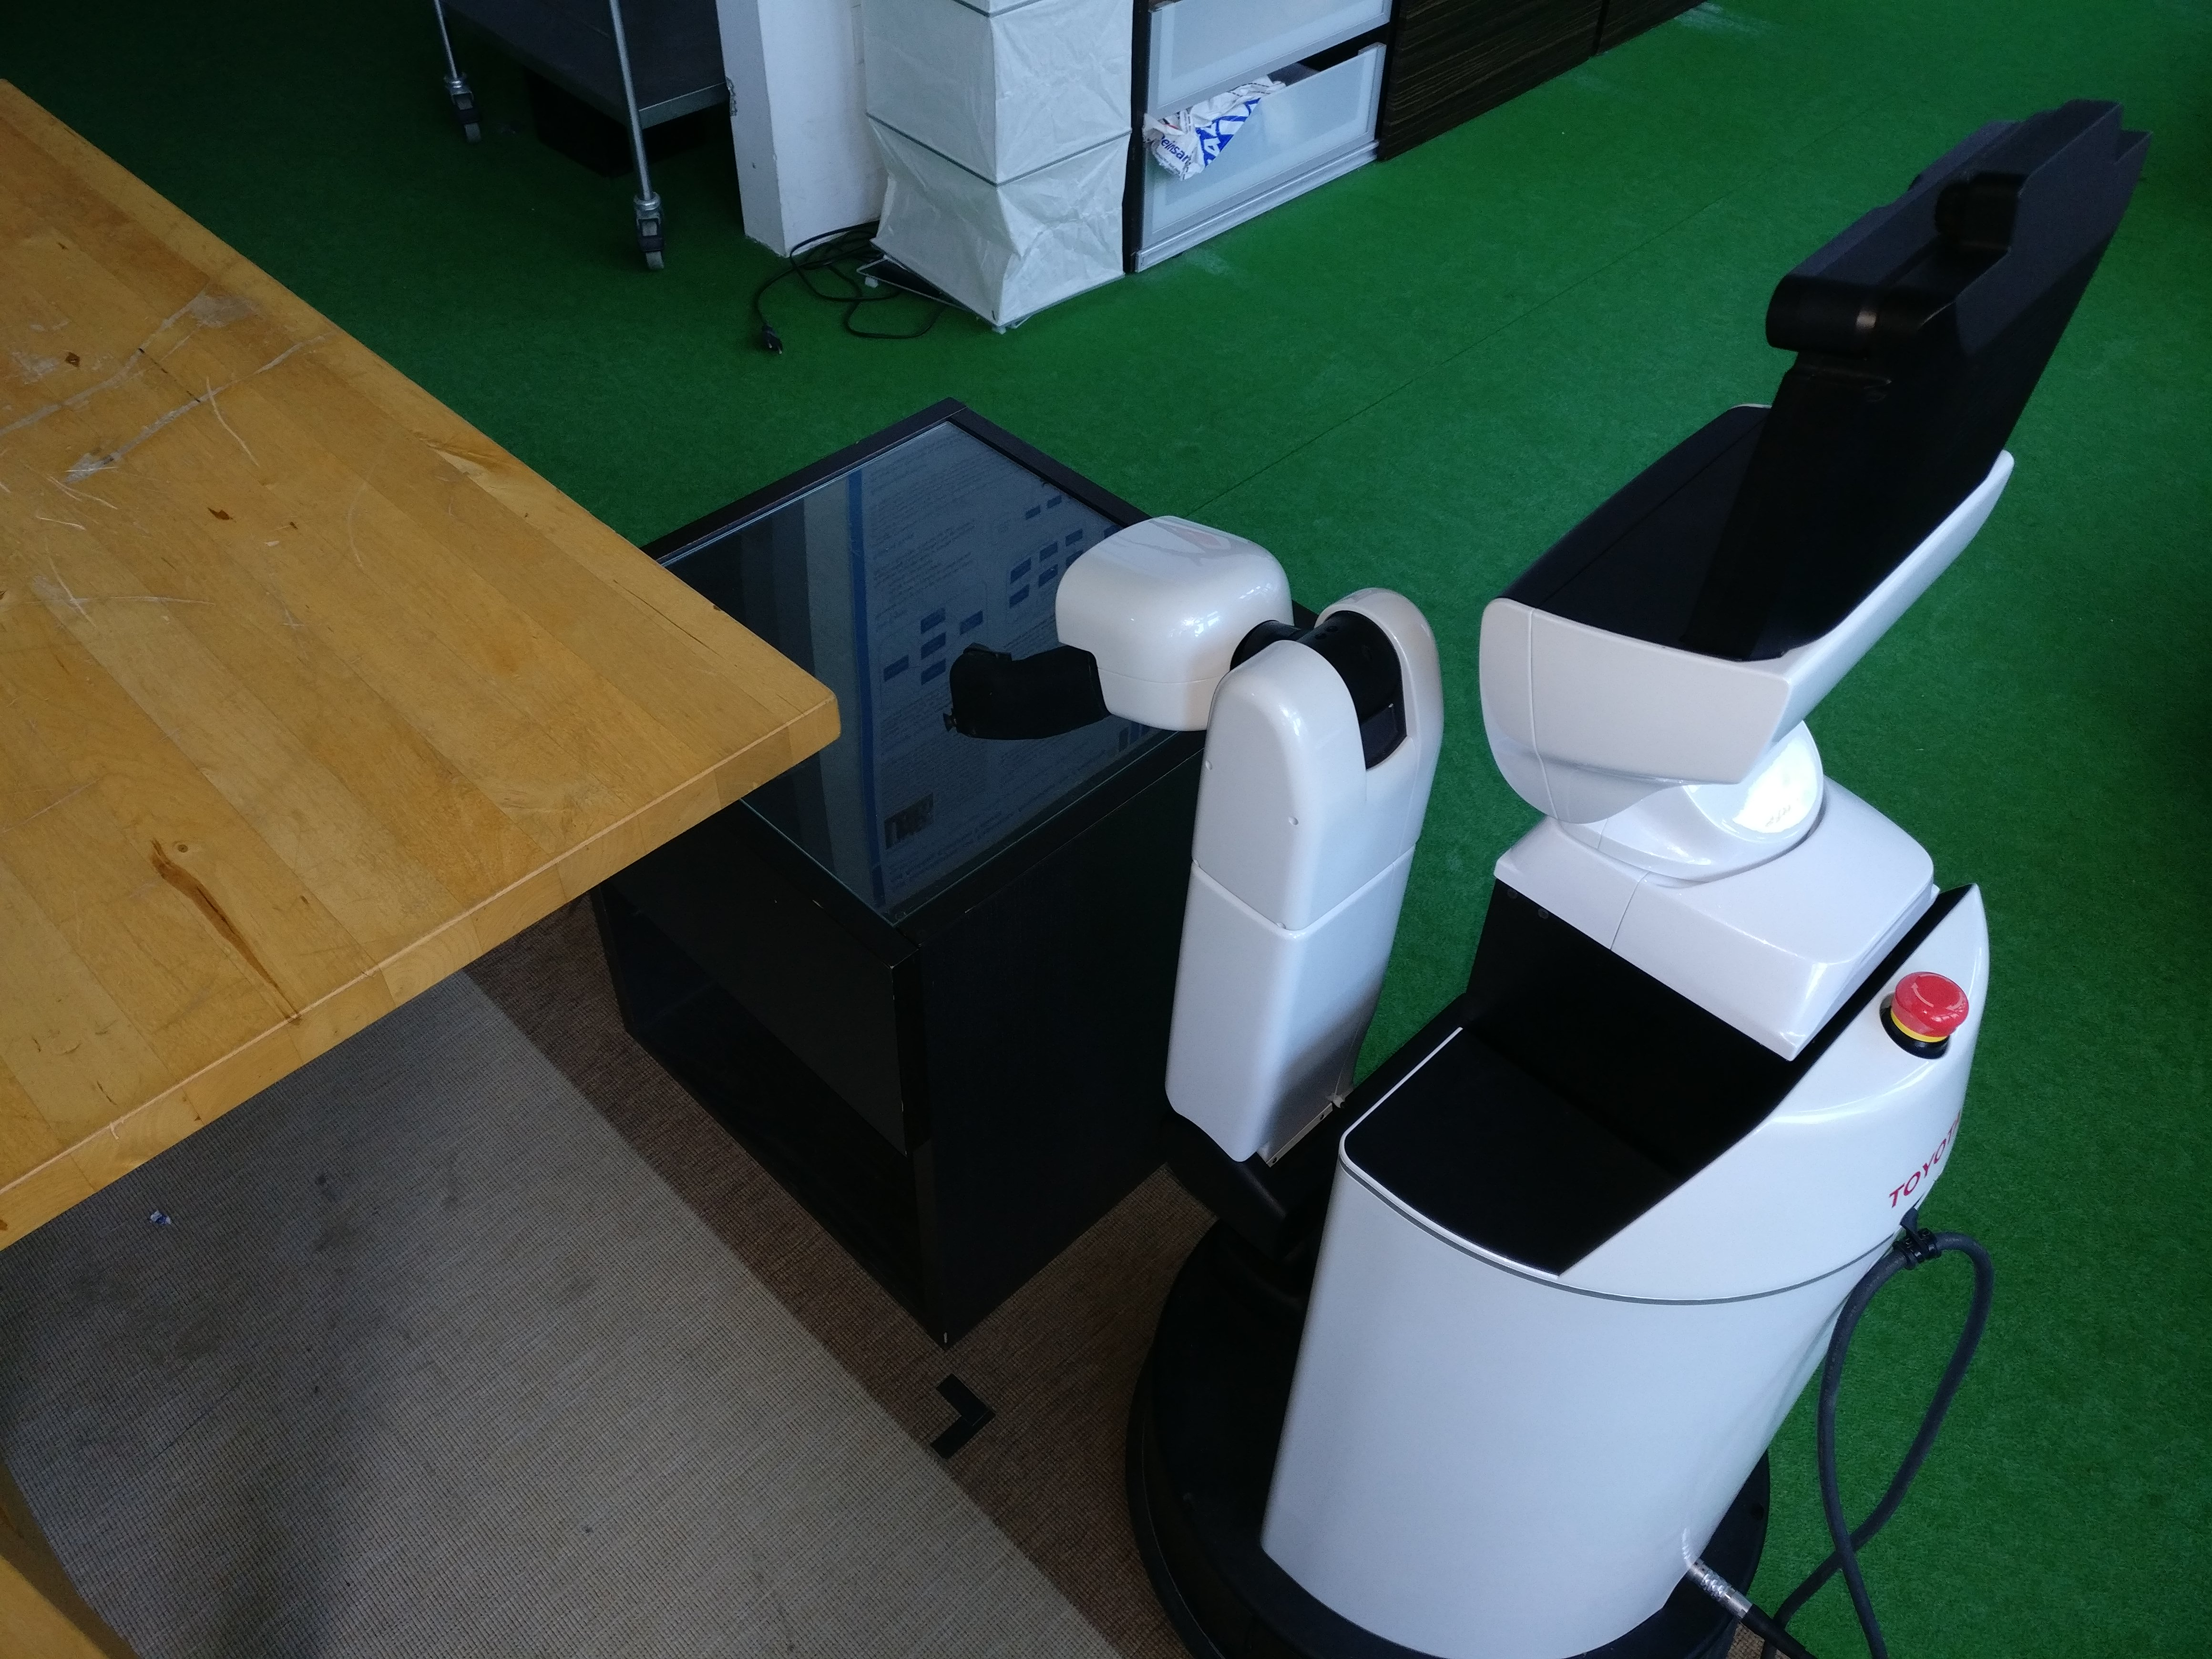
\includegraphics[scale=0.07]{images/multi_dmp.jpg}
	\caption{Toyota HSR performing pick and place task}
	\label{fig:multi_dmp}
\end{figure}
In this experiment, two motion primitives were demonstrated to the robot; one for reaching to the object in straight line from a fixed initial position and another for placing that object on the table. These two motion primitives can be seen in fig. \ref{fig:sequence_0} as well as in \ref{fig:sequence_1} from a different angle.

The learned motion primitives were used to pick a hypothetical object from a low height table and place on a relatively taller table (height = 0.78$m$). Thirteen trials were conducted for same picking and placing position. Trajectory 1 in fig. \ref{fig:sequence_0} is for reaching to the object and trajectory 2 is for transporting the object to the placing location. 

Fig. \ref{fig:sequence_0_e} and \ref{fig:sequence_11_e} shows the error in the execution of the generated trajectories in each trial. The error is here is relatively higher as compared to the KUKA YouBot. The reason behind it is the joint velocity controller in Toyota HSR; which is an emulated pseudo joint velocity controller which uses joint position controller to implement the joint velocity control, hence it does not provide precise velocity control.   

\begin{figure}[H]
	\centering
	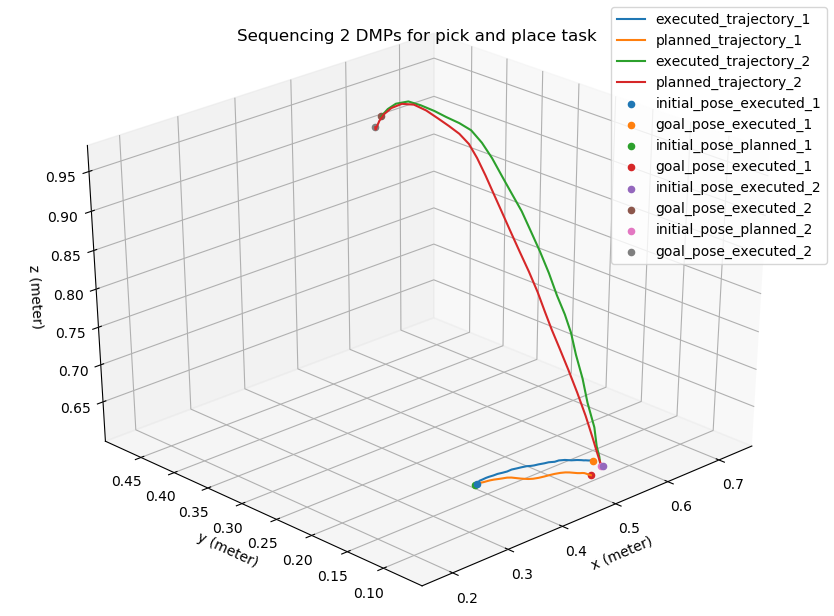
\includegraphics[scale=0.55]{images/HSR_3/sequence.png}
	\caption{Sequencing two DMPs for pick and place task - 1}
	\label{fig:sequence_0}
\end{figure}

\begin{figure}[H]
	\centering
	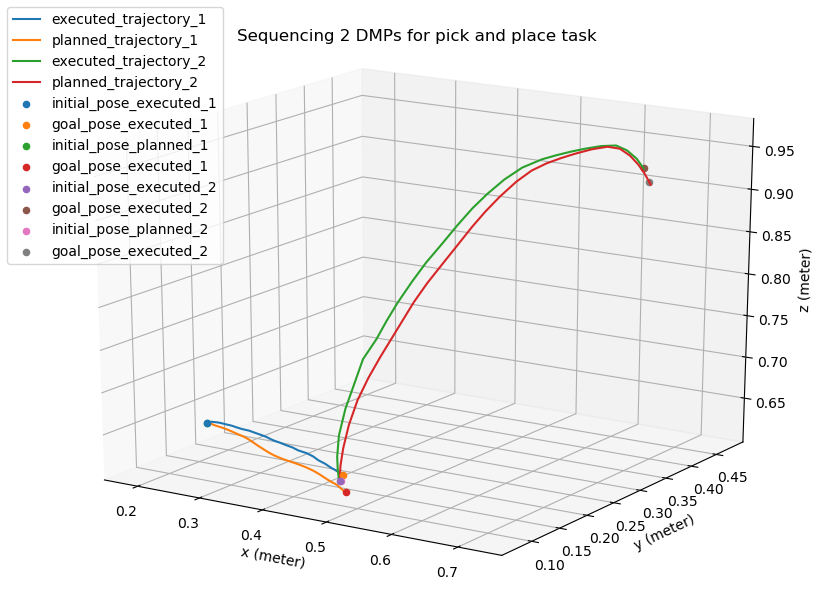
\includegraphics[scale=0.55]{images/HSR_3/sequence_1.png}
	\caption{Sequencing two DMPs for pick and place task - 2}
	\label{fig:sequence_1}
\end{figure}


\begin{figure}[H]
	\centering
	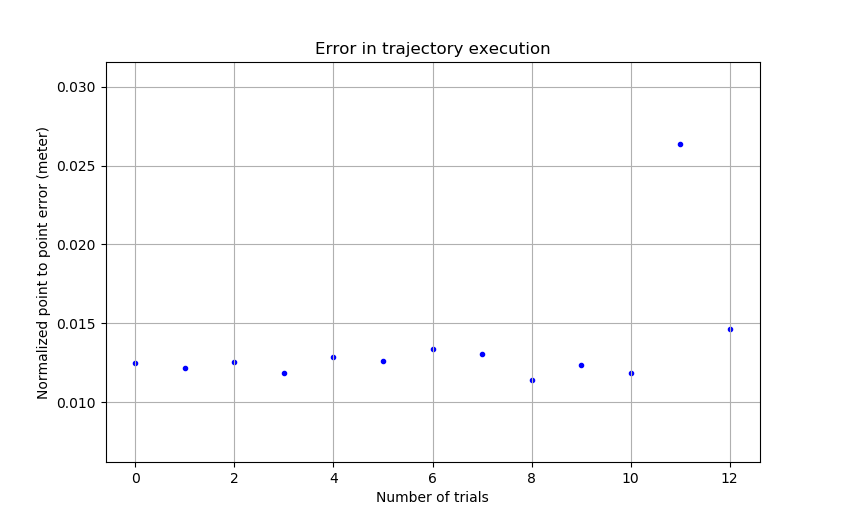
\includegraphics[scale=0.6]{images/HSR_3/sequence_0_e.png}
	\caption{Error in execution of trajectory 1}
	\label{fig:sequence_0_e}
\end{figure}


\begin{figure}[H]
	\centering
	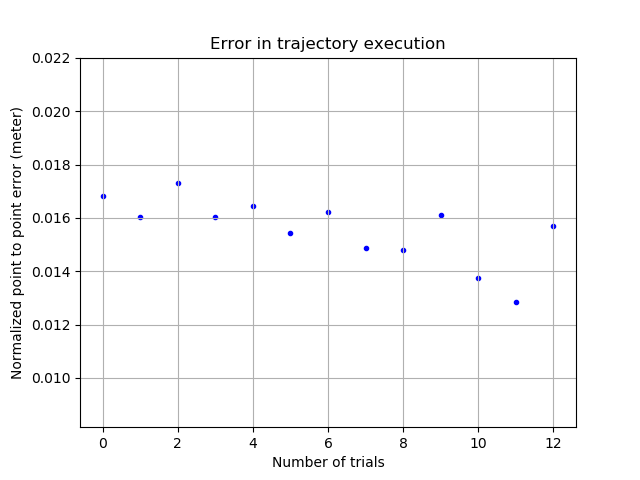
\includegraphics[scale=0.7]{images/HSR_3/sequence_1_e.png}
	\caption{Error in execution of trajectory 2}
	\label{fig:sequence_11_e}
\end{figure}


\subsection{Grasping an object}

\begin{figure}[H]
	\centering
	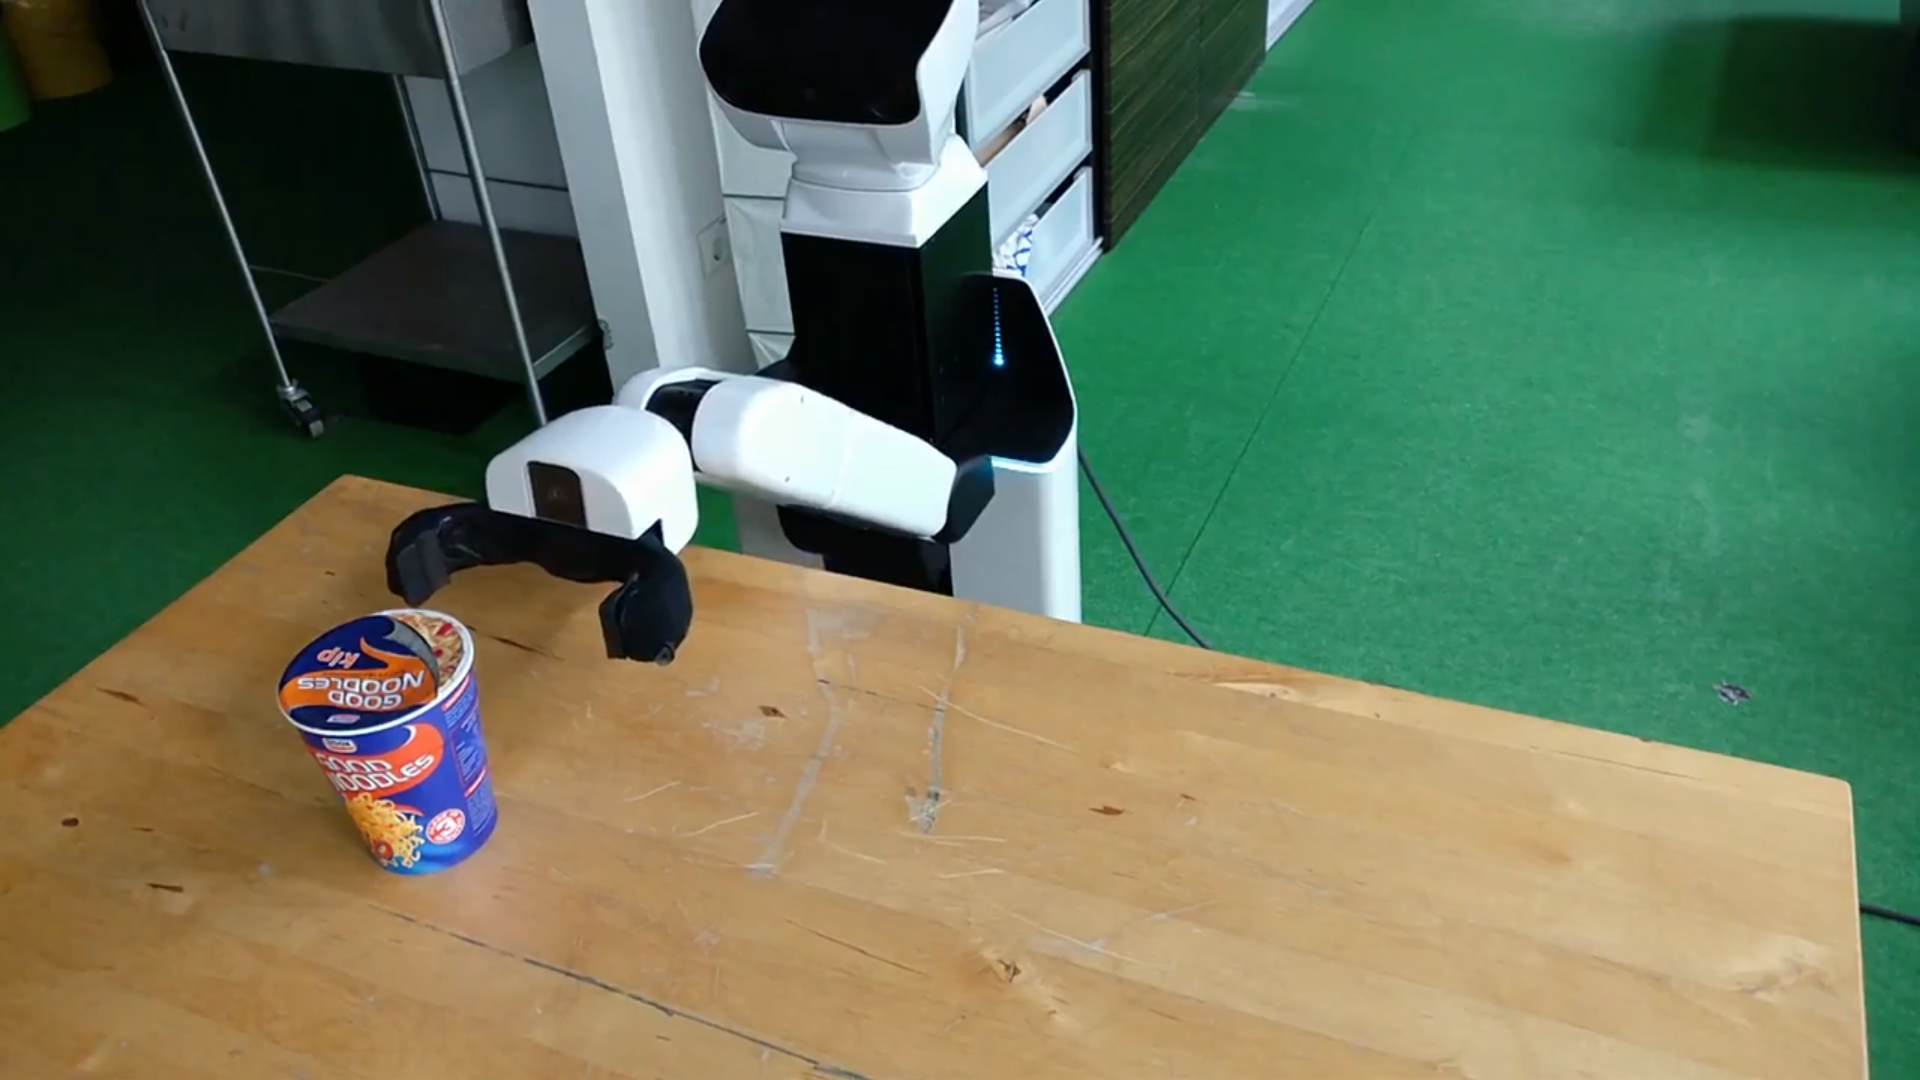
\includegraphics[width=\textwidth]{images/object_grasp.png}
	\caption{Toyota HSR grasping noodle box}
	\label{fig:object_grasp}
\end{figure}

Following figures show the performance of DMP framework integrated in current \textit{move\_arm} action server used in Toyota HSR. In this experiment, actual poses of the objects were obtained with the help of perception pipeline, and DMPs were used to generate the trejectories for grasping these objects. DMP generated trajectories for every goal given as opposed to the MoveIt! motion planning architecture, where solutions were not generated most of the time as the object was not in the reach of the arm. Execution of the trajectories generated by DMP was possible because of the whole body motion. In this experiment, executed trajectories show relatively higher deviations from planned trajectories. This happened because of the low update rate of the end-effector position. Error in the trajectory execution, shown in \ref{fig:grasp_e}, is relatively low and hence all the grasps were successful. 

\begin{figure}[H]
	\centering
	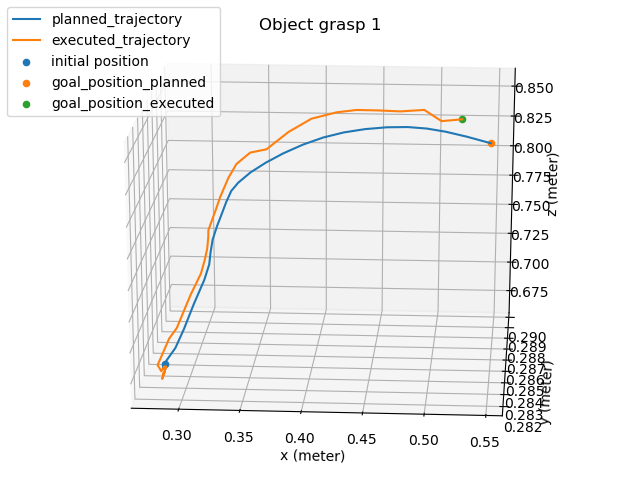
\includegraphics[scale=0.7]{images/HSR_4/1.png}
	\caption{Grasp 1}
	\label{fig:grasp_1}
\end{figure}

\begin{figure}[H]
	\centering
	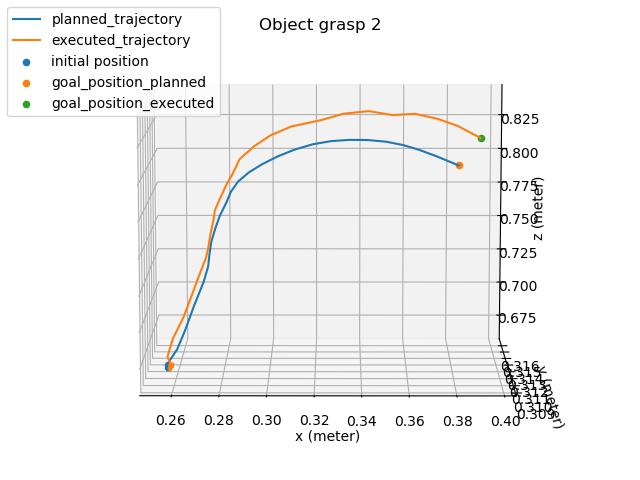
\includegraphics[scale=0.7]{images/HSR_4/2.png}
	\caption{Grasp 2}
	\label{fig:grasp_2}
\end{figure}

\begin{figure}[H]
	\centering
	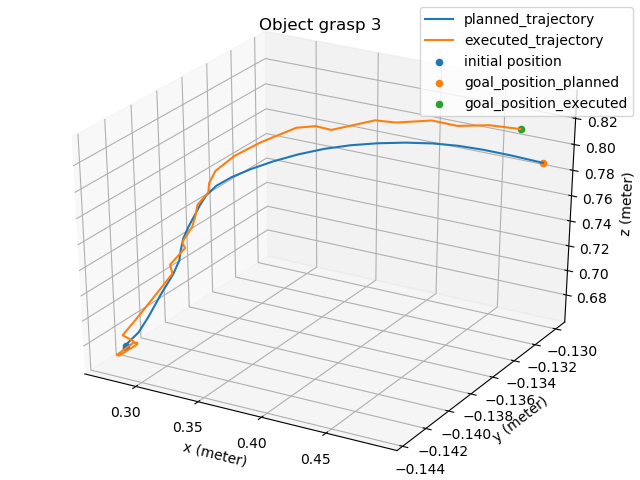
\includegraphics[scale=0.7]{images/HSR_4/3.png}
	\caption{Grasp 3}
	\label{fig:grasp_3}
\end{figure}

\begin{figure}[H]
	\centering
	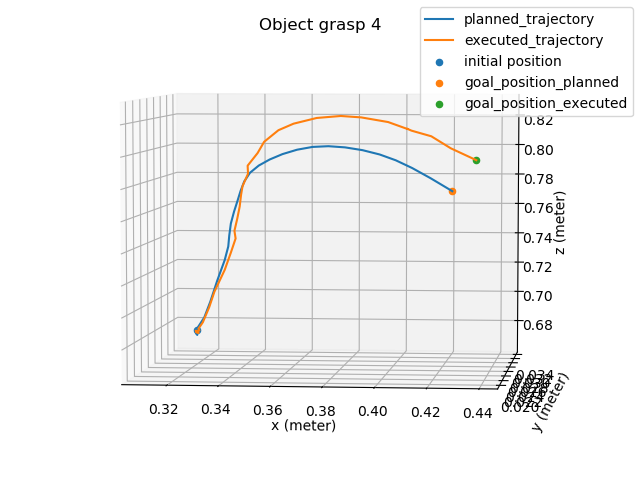
\includegraphics[scale=0.7]{images/HSR_4/4.png}
	\caption{Grasp 4}
	\label{fig:grasp_4}
\end{figure}

\begin{figure}[H]
	\centering
	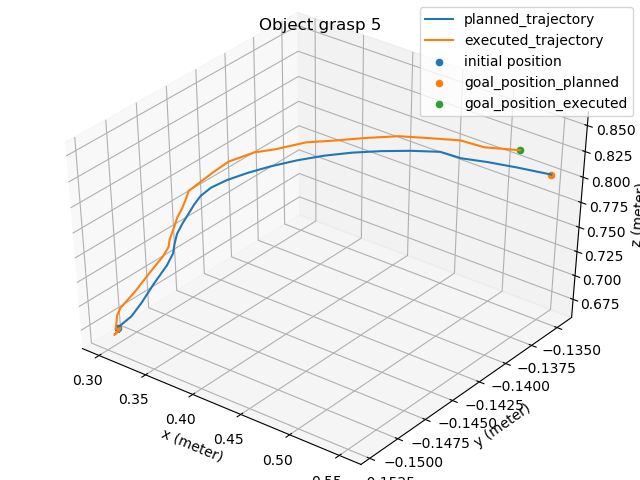
\includegraphics[scale=0.7]{images/HSR_4/5.png}
	\caption{Grasp 5}
	\label{fig:grasp_5}
\end{figure}


\begin{figure}[H]
	\centering
	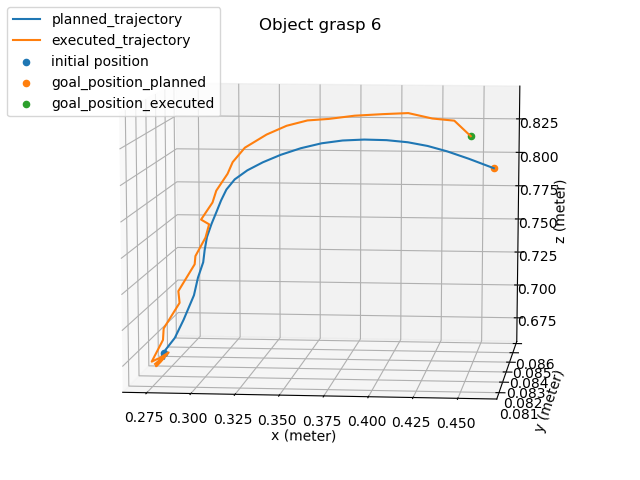
\includegraphics[scale=0.7]{images/HSR_4/6.png}
	\caption{Grasp 6}
	\label{fig:grasp_6}
\end{figure}


\begin{figure}[H]
	\centering
	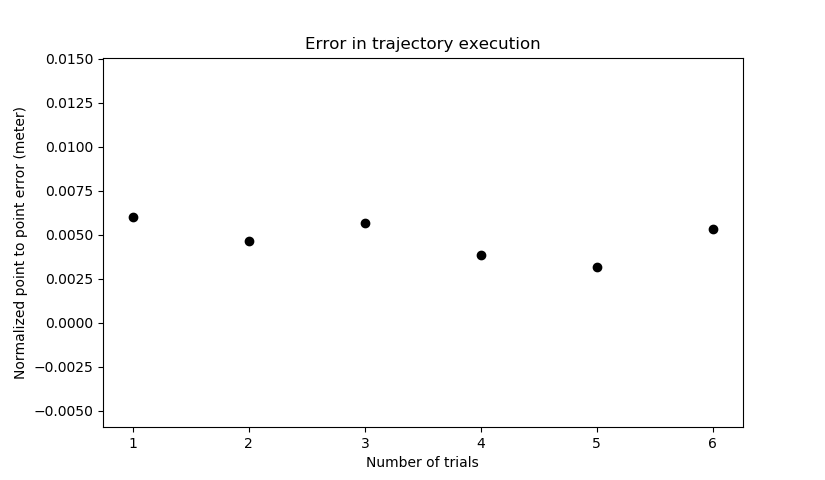
\includegraphics[scale=0.7]{images/HSR_4/e.png}
	\caption{Error in execution of grasping trajectories}
	\label{fig:grasp_e}
\end{figure}

While performing the experiments, test reports were maintained so that these experiments can be reproduced if needed. Test reports contain all the necessary data describing experiment and experimental conditions. These test reports can be found in Appendix section. 
